%%%%%%%% ICML 2026 EXAMPLE LATEX SUBMISSION FILE %%%%%%%%%%%%%%%%%

\documentclass{article}

% Recommended, but optional, packages for figures and better typesetting:
\usepackage{microtype}
\usepackage{graphicx}
\usepackage{subcaption}
\usepackage{booktabs} % for professional tables

% hyperref makes hyperlinks in the resulting PDF.
% If your build breaks (sometimes temporarily if a hyperlink spans a page)
% please comment out the following usepackage line and replace
% \usepackage{icml2026} with \usepackage[nohyperref]{icml2026} above.
\usepackage{hyperref}


% Attempt to make hyperref and algorithmic work together better:
\newcommand{\theHalgorithm}{\arabic{algorithm}}

% Use the following line for the initial blind version submitted for review:
\usepackage[accepted]{icml2026}

% For theorems and such
\usepackage{amsmath}
\usepackage{amssymb}
\usepackage{mathtools}
\usepackage{amsthm}

% if you use cleveref..
\usepackage[capitalize,noabbrev]{cleveref}

\input{math_commands}
\usepackage{xcolor}
\newcommand{\fazl}[1]{%
  \textcolor{orange}{\textbf{[Fazl: #1]}}\\
}

% if you use cleveref..
\usepackage[capitalize,noabbrev]{cleveref}

%%%%%%%%%%%%%%%%%%%%%%%%%%%%%%%%
% THEOREMS
%%%%%%%%%%%%%%%%%%%%%%%%%%%%%%%%
\theoremstyle{plain}
\newtheorem{theorem}{Theorem}[section]
\newtheorem{proposition}[theorem]{Proposition}
\newtheorem{lemma}[theorem]{Lemma}
\newtheorem{corollary}[theorem]{Corollary}
\theoremstyle{definition}
\newtheorem{definition}[theorem]{Definition}
\newtheorem{assumption}[theorem]{Assumption}
\theoremstyle{remark}
\newtheorem{remark}[theorem]{Remark}

% Todonotes is useful during development; simply uncomment the next line
%    and comment out the line below the next line to turn off comments
%\usepackage[disable,textsize=tiny]{todonotes}
\usepackage[textsize=tiny]{todonotes}

% The \icmltitle you define below is probably too long as a header.
% Therefore, a short form for the running title is supplied here:
\icmltitlerunning{Quantifying the Effect of Test Set Contamination on Generative Evaluations}

\begin{document}

\twocolumn[
  \icmltitle{Quantifying the Effect of Test Set Contamination on Generative Evaluations}

  % It is OKAY to include author information, even for blind submissions: the
  % style file will automatically remove it for you unless you've provided
  % the [accepted] option to the icml2026 package.

  % List of affiliations: The first argument should be a (short) identifier you
  % will use later to specify author affiliations Academic affiliations
  % should list Department, University, City, Region, Country Industry
  % affiliations should list Company, City, Region, Country

  % You can specify symbols, otherwise they are numbered in order. Ideally, you
  % should not use this facility. Affiliations will be numbered in order of
  % appearance and this is the preferred way.
  \icmlsetsymbol{equal}{*}

  \begin{icmlauthorlist}
\icmlauthor{Rylan Schaeffer}{equal,stanfordcs}
\icmlauthor{Joshua Kazdan}{equal,stanfordstatistics}
\icmlauthor{Baber Abbasi}{eleutherai}
\icmlauthor{Ken Ziyu Liu}{stanfordcs}
\icmlauthor{Brando Miranda}{stanfordcs}
\icmlauthor{Ahmed Ahmed}{stanfordcs}
\icmlauthor{Fazl Barez}{oxford,martian}
\icmlauthor{Abhay Puri}{servicenow}
\icmlauthor{Niloofar Mireshghallah}{cmu}
\icmlauthor{Sanmi Koyejo}{stanfordcs}
\end{icmlauthorlist}

\icmlaffiliation{stanfordcs}{Stanford Computer Science}
\icmlaffiliation{stanfordstatistics}{Stanford Statistics}
\icmlaffiliation{oxford}{University of Oxford}
%\icmlaffiliation{whitebox}{White Box}
\icmlaffiliation{martian}{Martian}
\icmlaffiliation{servicenow}{ServiceNow Research}
\icmlaffiliation{cmu}{Carnegie Mellon University}
\icmlaffiliation{eleutherai}{EleutherAI}

\icmlcorrespondingauthor{Rylan Schaeffer}{rschaef@cs.stanford.edu}
\icmlcorrespondingauthor{Joshua Kazdan}{jkazdan@stanford.edu}
\icmlcorrespondingauthor{Niloofar Mireshghallah}{nmireshg@andrew.cmu.edu}
\icmlcorrespondingauthor{Sanmi Koyejo}{sanmi@cs.stanford.edu}


  % You may provide any keywords that you find helpful for describing your
  % paper; these are used to populate the "keywords" metadata in the PDF but
  % will not be shown in the document
  \icmlkeywords{Test Set Contamination, Test Set Leakage, Scaling Laws, Memorization, Machine Learning, ICML}

  \vskip 0.3in
]

% this must go after the closing bracket ] following \twocolumn[ ...

% This command actually creates the footnote in the first column listing the
% affiliations and the copyright notice. The command takes one argument, which
% is text to display at the start of the footnote. The \icmlEqualContribution
% command is standard text for equal contribution. Remove it (just {}) if you
% do not need this facility.

% Use ONE of the following lines. DO NOT remove the command.
% If you have no special notice, KEEP empty braces:
\printAffiliationsAndNotice{}  % no special notice (required even if empty)
% Or, if applicable, use the standard equal contribution text:
% \printAffiliationsAndNotice{\icmlEqualContribution}

\begin{abstract}
    Test set contamination -- the inclusion of benchmarks in pretraining data -- has emerged as a critical threat to the trustworthy evaluation of frontier AI systems  
    While research has thoroughly investigated the impact of test set contamination on \emph{discriminative} evaluations, comparatively little research has studied the impact of test set contamination on \emph{generative} evaluations.
    In this work, we quantitatively assess the effects of test set contamination on generative evaluations through the language model lifecycle.
    We pretrain language models on mixtures of web data and the MATH benchmark, sweeping model sizes and number of test set replicas contaminating the pretraining corpus; performance improves with contamination and model size.
    Using scaling laws, we make a surprising discovery: including even a single test set replica enables models to achieve lower loss than the irreducible error of training on the uncontaminated corpus.
    We then study further training: overtraining with fresh data reduces the effects of contamination, whereas supervised finetuning on the training set will increase performance for low contamination but decrease performance for high contamination.
    Finally, at inference, we identify factors that modulate memorization: high sampling temperatures mitigate contamination effects, and longer solutions are exponentially more difficult to memorize than shorter ones, presenting a contrast with discriminative evaluations, where solutions are only a few tokens in length.
    By characterizing how generation and memorization interact, we highlight new considerations for trustworthy evaluation of AI systems.
\end{abstract}


\section{Introduction}
\label{sec:introduction}

As frontier AI systems are pretrained on web-scale data, test set contamination has become a critical concern for accurately assessing their capabilities \citep{sainz2023nlp,schaeffer2023pretrainingtestsetneed,xu2024benchmarkdatacontaminationlarge,deng2024unveiling,reuel2025open}. 
Evaluation aims to measure generalization on tasks the model has never seen, yet the sheer scale of modern pretraining makes such contamination increasingly likely \citep{brown2020language, du2022glam, wei2022finetuned,chowdhery2022palmscalinglanguagemodeling,touvron2023llama2openfoundation}. 

Prior research has sought to quantify the impact of test set contamination, also known as leakage, through two primary lenses. \textit{Statistical approaches} attempt to detect contamination or estimate its influence by modifying the test set, for example, by reordering, rephrasing, or replicating benchmark problems, e.g., \citep{oren2023proving, ni2025trainingbenchmarkneed, shi2024detecting, golchin2023data,golchin2024time,roberts2024to, wang2025generalization, zhang2024carefulexaminationlargelanguage}.
In comparison, \textit{controlled approaches} -- which offer the most rigorous measurement -- intentionally contaminate pretraining corpora to quantify how specific dosages of leakage inflate performance, e.g., \citep{magar2022data,jiang2024investigatingdatacontaminationpretraining,oren2023proving,yao2024data, wang2025generalization,kocyigit2025overestimation,bordt2025howmuch}.
For a more thorough discussion, please see Appendix~\ref{app:sec:related_work} Related Work.

\begin{figure*}[t!]
\centering
\hspace{-1em}
\begin{minipage}[t]{0.47\textwidth}
    \vspace{0pt}
    \centering
    % \includegraphics[width=\linewidth]{figures/01_revised_figures/pretraining_schematic.png}
    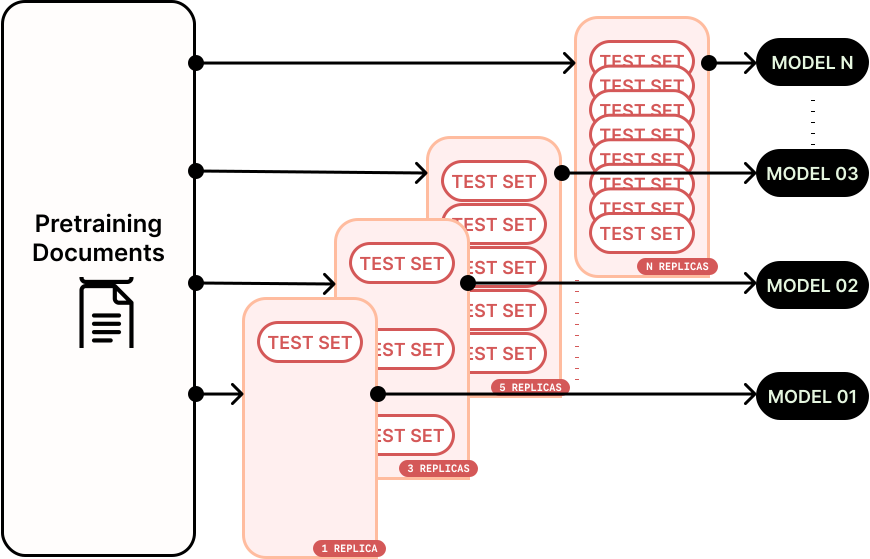
\includegraphics[width=\linewidth]{figures/schematic.pdf}
\end{minipage}%
\hspace{0.1em}
\begin{minipage}[t]{0.49\textwidth}
    \vspace{0pt}
    \centering
    \includegraphics[width=\linewidth]{figures/11_math_qwen3_pt_math_verify/y=math_verify_by_num_parameters_by_num_replicas.pdf}    
    % \includegraphics[width=\linewidth]{figures/10_math_qwen3_pt_cross_entropy/y=loss_by_num_parameters_by_num_replicas.pdf}
    \includegraphics[width=\linewidth]{figures/10_math_qwen3_pt_cross_entropy/y=loss_ratio_by_num_parameters_by_num_replicas.pdf}
\end{minipage}
    \caption{\textbf{Performance on Generative Benchmarks Increases with Test Set Contamination and Model Size.} \text{Schematic:} We pretrained compute-optimal language models ($34$M--$344$M parameters) on corpora containing different replicas of the MATH test set ($0$--$3162$). Evaluation used greedy decoding (temperature $=0$). \textbf{Left:} As contamination (quantified by the number of test set replicas in the pretraining corpus) increases, Math Verify scores (top) rise and cross entropies on the test set (bottom) fall, consistent with discriminative evaluations, with a sharp improvement around $100$. \textbf{Right:} The ratio in the loss on the MATH test set between $R$ replicas and $0$ replicas grows with model size, meaning larger models benefit more from test set contamination for the same number of replicas (consistent with prior findings that larger models memorize more readily \citep{tirumala2022memorization, carlini2023quantifying, biderman2023emergent}; see Appendix~\ref{app:sec:related_work}).}
    \label{fig:math_verify_ce_temp_0}
\end{figure*}

While foundational, these investigations have predominantly focused on \textit{discriminative} benchmarks like classification or multiple-choice question-answering (MCQA). For example, \citet{magar2022data} used SST-2 \citep{socher2013sst} (classification). \citet{jiang2024investigatingdatacontaminationpretraining} used SST-2 (classification), MMLU \citep{hendrycks2021measuring} (MCQA), SQuAD \citep{rajpurkar2016squad} (MCQA), and CNN/Daily Mail (fill-in-the-middle) \citep{nallapati2016abstractive}. \citet{oren2023proving} used 7 MCQA benchmarks and 1 mathematical problem solving benchmark (GSM8K) \citep{cobbe2021trainingverifierssolvemath}, \citet{yao2024data} used 3 MCQA benchmarks while \citet{bordt2025howmuch} used 7 MCQA benchmarks.

However, with the rapid advancement of model capabilities and the advent of reasoning models \citep{openai2024openaio1card,comanici2025gemini25pushingfrontier,xu2025largereasoningmodelssurvey}, the field is shifting towards benchmarks for which the model must generate an answer rather than choose between provided answers.
Whether test set contamination has the same effect on generative evaluation as on discriminative evaluations is unclear.
Discriminative evaluations typically require the model to place higher probability mass on the correct choice than on a small number of alternative incorrect choices \citep{gao2024evalharness, schaeffer2025elusive}, and candidate choices are often only a couple of tokens long.
In contrast, generative evaluations require the model to produce solutions spanning tens-to-thousands of tokens without straying from the memorized path, and introduce new considerations such as the sampling temperature \citep{ackley1985learning}, the sampling algorithm (e.g., top-k \citep{fan2018topk}, top-p \citep{holtzman2020topp}) and the solution length.


\begin{figure*}[t!]
    \centering
    \includegraphics[width=0.9\linewidth]{figures/20_gen_eval_contamination_vs_compute/y=loss_x=flop_hue=num_replicas.pdf}
    \includegraphics[width=0.9\linewidth]{figures/20_gen_eval_contamination_vs_compute/y=fit-params_x=num-replicas_col=param_setting=full-fits.pdf}
    \caption{\textbf{Scaling Laws Suggest Including A Single Test Set Replica Achieves Lower Loss Than the Irreducible Error of the Uncontaminated Corpus.} \textbf{Top:} For each scaling series pretrained on corpora contaminated with $R$ replicas of the MATH test set, we fit scaling laws $\mathcal{L}(C, R) = E(R) + C_0(R) \cdot C^{-\alpha(R)}$, where $C=6\, N \, D$ is the pretraining compute. 
    Almost all contaminated models achieve lower cross entropy on the MATH test set than the irreducible error of training on uncontaminated data (horizontal purple line).
    \textbf{Bottom:} Increasing test set contamination reduces the irreducible error $E(R)$ from $3.594$ at $R=0$ to $0.0347$ at $R=316$. Larger values of $R$ also increase the compute prefactor and compute exponent.
    The functional form achieves average fitting error $< 10^{-2}$ for all $R$.
    }
    \label{fig:contamination_scaling_laws}
\end{figure*}

In this work, we quantitatively study the effects of test set contamination on generative evaluations, focusing on the widely used MATH benchmark \citep{hendrycks2021measuringmathematicalproblemsolving}. 
We pretrain dozens of language models on corpora contaminated with varying numbers of test set replicas, sweeping across model sizes, sampling temperatures, and token budgets. 
% Our findings reveal that while generative contamination shares some similarities with discriminative settings, it introduces new interactions between memorization and generalization.
We make the following contributions:
%
\begin{itemize}
    \item \textbf{Pretraining (Scaling \& Irreducible Error):} We quantify how contamination impacts pretrained models. We find that performance increases with the number of test set replicas in the pretraining corpus and with model size, similar to discriminative settings. Under standard scaling law assumptions, we discover that including even a single replica of the test set enables models to achieve a lower loss than the estimated irreducible error of the uncontaminated corpus.
    
    \item \textbf{Further Training (Overtraining \& Supervised Finetuning):} We find that training beyond compute-optimal with fresh data dilutes increased performance from contamination, similar to discriminative settings. We then show that SFT on the training data has opposing effects, depending on the amount of contamination in pretraining: performance improves for low contamination, but worsens for high contamination.

    \item \textbf{Inference (Temperature \& Solution Length):} We identify distinct factors that modulate memorization during generation: increasing sampling temperature and increasing solution sequence length each reduce model performance, as models struggle to regurgitate long sequences without decohering.

    \item \textbf{Correction to Evaluation Library:} We identify and fix a critical implementation error in the widely used EleutherAI LM Evaluation Harness \citep{gao2024evalharness} for Math Verify Scores. Our correction ensures that valid reference solutions are accurately scored as correct (raising gold reference solutions' scores from $\mathord{\sim}$70\% to 100\%), a necessary step for trustworthy reporting on mathematical benchmarks.
\end{itemize}


\section{Methodology}
\label{sec:methodology}

\textbf{Pretraining} To study the effects of contamination in generative evaluations, we pretrained transformer-based \citep{vaswani2017attention} causal language models from initialization using the Qwen 3 architecture \citep{yang2025qwen3technicalreport}, sweeping model sizes: $34$M, $62$M, $93$M, $153$M, $344$M.
Following Chinchilla compute-optimal scaling \citep{hoffman2022chinchilla}, each model was pretrained with 20 tokens-per-parameter.
For each model size and token budget, we created multiple pretraining corpora by contaminating a high quality web crawl corpus \citep{penedo2024finewebdatasetsdecantingweb} with a different number of replicas of the benchmark test set: from $0$ (uncontaminated) through $1, 3, 10, 32, 100, 316, 1000, 3162$ (uniformly spaced on a log scale).
Pretraining compute was calculated using the common approximation $C \approx 6  \, N \, D$ \citep{kaplan2020scaling,sardana2024beyond,porian2024resolving,gadre2024languagemodelsscalereliably}, where $N$ is model parameters and $D$ is pretraining tokens.
For implementation details, see Appendix~\ref{app:sec:pretraining_implementation_details}.

\textbf{Benchmark} We chose the ubiquitous MATH \citep{hendrycks2021measuringmathematicalproblemsolving} benchmark of competition math problems.  The MATH dataset has several properties that made it our benchmark of choice: it is comparatively large \fazl{szie?}, the answers are easy to verify, and the benchmark includes solutions as well as answers. 
These solutions exhibit high variability in both length and difficulty.
The MATH test set contains $\mathord{\sim}1.4$M tokens under the Qwen 3 tokenizer.


\textbf{Evaluation} 
We evaluated our models using two metrics. The first metric we report is \emph{Math Verify}, defined as the fraction of problems for which the model generates solutions that are verified to be mathematically equivalent to the benchmark's boxed answers.
We initially evaluated our models using EleutherAI's Language Model Evaluation Harness \citep{gao2024evalharness}, but discovered an error with how Math Verify scores are computed; for example, the benchmark's gold reference solutions obtained a Math Verify score around 70\%.
\href{https://github.com/EleutherAI/lm-evaluation-harness/issues/3210}{We worked with its developers to correct the implementation}. \fazl{maybe fully write the issue and solution in appendix as this is nice finding and papers from 1+ year may want to correct} As an aside, this suggests to us that any research reporting MATH scores from the past 1+ years may have reported incorrect scores.
The second metric we report is the \emph{Cross Entropy} of the gold reference solutions given the problems, which were previously demonstrated to be useful for studying scaling properties of generative evaluations during pretraining \citep{schaeffer2025pretrainingscalinglawsgenerative}.
We used temperature-only sampling, beginning with temperature $0$ (``greedy''), and expanding to more temperatures in Sec.~\ref{sec:temperature}.
\section{Pretraining: Scaling \& Irreducible Error}
\label{sec:pretraining}

We begin at the first stage of the model lifecycle: pretraining.
We establish foundational results on how test set contamination interacts with model scale and compute, and use scaling laws to quantify what contamination ``buys'' a model.

\begin{figure*}[t!]
    \centering
    \includegraphics[width=\linewidth]{figures/10_math_qwen3_pt_cross_entropy/y=loss_x=num_replicas_hue=ot_col=params.pdf}
    \includegraphics[width=\linewidth]{figures/10_math_qwen3_pt_cross_entropy/y=loss_x=ot_hue=num_replicas_col=params.pdf}
    \caption{\textbf{Overtraining with Fresh Data Mitigates Contamination.} Consistent with discriminative evaluations \citep{bordt2025howmuch}, we find an interaction between contamination and overtraining (i.e., training longer than Chinchilla compute-optimal; Eqn.~\ref{eqn:overtrain_multiplier}) on \emph{new fresh data}. For models with low contamination, cross entropy on the MATH test set decreases with increasing overtraining; however, for models with high contamination, cross entropy increases with overtraining. This suggests that while fresh data generally improves performance, it dilutes the ``dose,'' or proportion of contaminated pretraining tokens, thereby lessening the effect of the contamination. The crossover point shifts with model size, falling from 32 test set replicas for 34M to 1 replica for 93M models, indicating larger models lose their contamination advantage more readily when overtrained.}
    \label{fig:overtraining}
\end{figure*}


\paragraph{Finding \#1: Performance Increases with Contamination and Model Size} Consistent with discriminative evaluations, increasing the number of benchmark replicas in the pretraining corpus increases Math Verify scores and decreases cross entropies (Fig.~\ref{fig:math_verify_ce_temp_0} Left), as does increasing model size (Fig.~\ref{fig:math_verify_ce_temp_0} Right).
We observe a non-linear relationship between the number of test set replicas and model performance:
For low levels of contamination ($\leq$ 10 replicas), the impact on performance is minimal, with Math Verify scores and cross entropies remaining close to uncontaminated performance; at around 100 replicas, performance sharply increases (Fig.~\ref{fig:math_verify_replicas_temp}).
At the highest levels of contamination, the model achieves ceiling performance.


\paragraph{Finding \#2: Scaling Laws Suggest Including A Single Test Set Replica Achieves Lower Loss Than the Irreducible Error of the Uncontaminated Corpus}

How much does test set contamination ``buy" the model in terms of performance? 
More specifically, how much pretraining compute must be spent on an uncontaminated pretraining corpus to match the performance of a model trained on a corpus containing $R$ replicas of the benchmark test set?

To answer this question, we turned to neural scaling laws.
Based on previous work \citep{kaplan2020scaling, hoffman2022chinchilla, openai2024gpt4technicalreport, hu2024predictingemergentabilitiesinfinite, schaeffer2025pretrainingscalinglawsgenerative}, for each scaling series pretrained on corpora contaminated with $R \in \{0, 1, 3, 10, 32, 100, 316\}$ replicas of the MATH test set, we fit neural scaling laws for the cross entropy loss $\mathcal{L}$ on the benchmark test set:
%
\begin{equation}
    \label{eqn:neural_scaling_law}
    \mathcal{L}(C, R) = E_0(R) + \frac{C_0(R)}{C^{\alpha(R)}},
\end{equation}
%
where $E_0(R) > 0$ is the irreducible error, $C_0(R) > 0$ is the compute prefactor and $\alpha(R) > 0$ is the compute exponent.


Fig.~\ref{fig:contamination_scaling_laws} shows each scaling law, as well as each scaling law's estimated parameters as a function of the number of test set replicas $R$.
Our models' pretraining compute budgets and losses on the test set are reasonably well fit by Eqn.~\ref{eqn:neural_scaling_law}, and the pretraining prefactors and pretraining exponents are roughly constant for the various values of $R$.
The biggest effect of increasing contamination is that the irreducible error shrinks from $E(R=0) = 3.594$ to $E(R=316) = 0.0347$.
On the models we trained, we found that \emph{including even a single replica enables almost all models to achieve lower cross entropy losses than the estimated irreducible error of the uncontaminated pretraining corpus}.
Under standard scaling law assumptions -- specifically, that the power-law form (Eqn.~\ref{eqn:neural_scaling_law}) extrapolates to infinite compute -- a contaminated pretraining corpus can buy more than an ``infinite'' amount of pretraining compute relative to pretraining on an uncontaminated pretraining corpus.


\begin{figure*}[t!]
    \centering
    \includegraphics[width=\linewidth]{figures/12_math_qwen3_sft_cross_entropy/combined_loss_analysis_hue=replicas_style=params.pdf}
    \caption{\textbf{Supervised Finetuning on the Train Set Has Opposing Effects, Depending on Pretraining Contamination.} For models pretrained with little-to-no contamination ($<10$ test set replicas), supervised finetuning (SFT) on the MATH \emph{train} set decreases loss on the \emph{test} set. For models pretrained with more contamination ($>10$ test set replicas), SFT on the train set increases loss on the test set.
    We conjecture that during SFT, contaminated models learn to generalize but also forget their contaminated pretraining data, and the effects of contaminated test set data are more impactful than generalization for small models, leading to a net increase in test loss. 
    }
    \label{fig:sft}
\end{figure*}

This conclusion potentially contradicts \citet{huang2024demystifying}'s claim that single-shot verbatim memorization is an ``illusion''  and \citet{hayes2025exploring}'s claim that membership inference attacks are limited on pre-trained LLMs, with AUC asymptoting to $\mathord{\sim}0.689$.
Future work should aim to understand this difference; one possible explanation is that MATH is distributionally different from FineWeb-Edu-Dedup in a way that makes identifying test set contamination easier.

\section{Further Training: Overtraining \& Supervised Finetuning (SFT)}
\label{sec:further_training}

\paragraph{Finding \#3: Overtraining with Fresh Data Mitigates Contamination} \fazl{fresh data sounds awkward for me - new data?}


\citet{bordt2025howmuch} recently reported that for discriminative evaluations, the effect of contamination diminishes when models are trained beyond the ``compute optimal'' ratio of 20 tokens-per-parameter \citep{hoffman2022chinchilla} on fresh data. We tested whether this so-called \emph{overtraining} \citep{touvron2023llama2openfoundation,sardana2024beyond,gadre2024languagemodelsscalereliably,schaeffer2025pretrainingscalinglawsgenerative} has similar effects for generative benchmarks.
We extended our Sec.~\ref{sec:methodology} pretraining sweep into the overtrained regime, pretraining on 
%
\begin{equation}\label{eqn:overtrain_multiplier}
D(m, N) \defeq m \times 20 \times N,
\end{equation}
%
tokens per model, where $m$ is the \emph{overtraining multiplier} and $N$ is the number of model parameters.
We swept $m \in \{1, 2, 4, 8, 16\}$.
Following \citet{sardana2024beyond,gadre2024languagemodelsscalereliably}, we term $m=1$ ``compute-optimal training'' and term $m > 1$ ``overtraining''.
Crucially, in \citet{bordt2025howmuch} and here, as the overtraining multiplier increases, the additional tokens are \emph{new fresh non-repeated tokens}; this differs from more practical settings where models might see select documents repeated tens-to-hundreds of times \citep{hernandez2022scalinglawsinterpretabilitylearning} or the entire corpus repeated for 4+ epochs \citep{muennighoff2023scaling,fang2025datasets}.

We find an interesting interaction between contamination and overtraining (Fig.~\ref{fig:overtraining}): for models with low contamination, cross entropy on the MATH test set decreases with increasing overtraining, but for models with high contamination, cross entropy on the MATH set increases with overtraining.
The cross-over point between test set replicas and overtraining multiplier shifts with model size: the crossover point falls from 32 test set replicas for $34$M parameter models to 10 replicas for $63$M parameter models to 1 replica for $93$M parameter models.
Thus, as models become larger, the performance boost from contamination diminishes when overtraining with fresh data.
Our interpretation is that while more fresh data is generally useful for improving model performance generally, it dilutes the ``dosage'' of the contaminated data, weakening how the model ``responds'' (as measured by task performance) \citep{schaeffer2025doseresponse}.

\paragraph{Finding \#4: Supervised Fine-Tuning on Training Set Has Opposing Effects, Depending on Pretraining Contamination}

After pretraining, the first post-training step is oftentimes supervised finetuning (SFT) \citep{wei2022finetunedlanguagemodelszeroshot, ouyang2022training}. We turned to assessing what effect, if any, SFT has on contaminated pretrained models. \citet{kocyigit2025the} recently studied this question and found that SFTing on the \emph{train} set improves performance on the \emph{test} set. However, as a key methodological difference, \citet{kocyigit2025the} induced test set contamination via continued pretraining \citep{jin2022lifelong,jang2022continualknowledgelearninglanguage,ibrahim2024simple, parmar2024reusedontretrainrecipe,yildiz2025investigatingcontinualpretraininglarge}, whereas we introduced test set contamination uniformly throughout pretraining.


\begin{figure*}[t!]
    \centering
    \includegraphics[width=\linewidth]{figures/11_math_qwen3_pt_math_verify/y=math_verify_x=num_replicas_hue=compute_col=temp.png}
    \caption{\textbf{Sampling Temperature Degrades Performance, Particularly for Contaminated Models.} 
    We report Math Verify scores as a function of test set replicas and model size across six sampling temperatures.
    As sampling temperature increases, Math Verify scores drop precipitously, falling from near 100\% to under 1\% in many configurations.
    The penalty for high temperature is disproportionately larger for highly contaminated models: increasing temperature from 0 to 1 reduces performance by a factor of $\sim2$ at low contamination levels ($\leq 10$ replicas), whereas it reduces performance by a factor of up to 40 at high contamination levels ($1000$ replicas).
    }
    \label{fig:math_verify_replicas_temp}
\end{figure*}

One might expect that SFTing on the train set should increase test set performance across the board.
We discover that, surprisingly, the opposite is sometimes true: SFTing on the train set can both help and hurt model performance on the test set, depending on the amount of contamination in pretraining (Fig.~\ref{fig:sft}).
For models with no or low $(< 10)$ test set contamination, SFTing on the train set significantly reduces loss on the test set (purple).
At $10$ test set replicas, SFT has no effect (aqua), but as contamination increases, SFTing on the train set significantly increases loss on the test set (yellow, green).
We conjecture that training highly contaminated models on the MATH train set causes forgetting of the test set in tandem with improved generalization.
As studied in Section \ref{eqn:neural_scaling_law}, the benefits of contamination on test loss dwarf those of generalization (which would be improved by SFT on the train set). 
Therefore, the net impact of SFTing on the train set for highly contaminated models is counterintuitively to increase cross entropy loss.
\section{Generation: Sampling Temperature and Solution Length}
\label{sec:temperature}


Generative benchmarks introduce distinct complexities compared to discriminative evaluations. Unlike multiple-choice tasks where predetermined sequences are score, generative solutions require the model to produce a coherent sequence over hundreds of tokens or more.
This introduces two critical levers for analyzing contamination: sampling temperature and solution length. In this section, we demonstrate that while contamination mimics reasoning capability under greedy decoding, this competence is brittle. We show that sampling and long-context requirements act as barriers that memorization struggles to overcome.

\paragraph{Finding \#5: High Temperature Sampling Mitigates the Gains from Contamination} 

We evaluated the pretrained models using temperature-only sampling, sweeping from $0$ (``greedy'') to $1.5$.
We observe that Math Verify scores remain stable between greedy decoding and low-temperature sampling ($\tau \leq 0.56$) (Fig.~\ref{fig:math_verify_replicas_temp}, left and center).
However, as temperature increases beyond this point, performance degrades quickly.

Crucially, higher temperature sampling acts as an equalizer, significantly reducing the performance gap between highly contaminated and uncontaminated models.
While uncontaminated models are bounded by a performance floor, contaminated models lose their memorization advantage under stochastic sampling.
For example, increasing temperature from $0$ to $1$ causes performance at high contamination levels ($1000$ replicas) to collapse by a factor of 40, bringing them much closer to the baseline performance of uncontaminated models.
This suggests that contamination-driven performance is brittle; small adjustments in inference settings can eliminate the effects of memorization almost entirely. 
High-temperature sampling flattens these peaks, causing the model to diverge from the memorized path and exposing the ``illusion'' of competence created by leakage.


\begin{figure*}[t!]
    \centering
    \includegraphics[width=\linewidth]{figures/11_math_qwen3_pt_math_verify/y=math_verify_x=solution_length_hue=num_replicas_col=temp_row=params_153M_344M.png}
    \caption{\textbf{Performance Declines with Increasing Solution Token Length.} Math Verify Scores decrease exponentially with solution length at high levels of benchmark replication. For lower levels of benchmark replication, score decreases appear to follow approximate power laws. Trends are consistent between the 153M and 344M parameter models. Shaded regions represent 95\% confidence intervals.
    }
    \label{fig:temp_and_solution_length}
\end{figure*}


\begin{figure*}[t!]
    \centering
    \includegraphics[width=\linewidth]{figures/11_math_qwen3_pt_math_verify/y=math_verify_x=loss_hue=temp_col=params_filtered.png}
    \caption{\textbf{Math Verify Score Is Correlated with Pretraining Loss.} Math Verify scores correlate strongly with the cross entropy loss achieved on the MATH Test Set during training, where differences in these graphs are attributable to increased repetition on the benchmark test set.  The correlation is significantly weaker for high temperatures, and falls to nearly $0$ for temperatures above $1$.  }
    \label{fig:loss_and_math_verify}
\end{figure*}


\paragraph{Finding \#6: Longer Solutions Reveal a Shift from Power Law to Exponential Decay} 

To understand how solution length constrains performance, we binned problems into 10 log-spaced intervals ranging from the shortest (15 tokens) to the longest (1949 tokens).
We find that Math Verify scores decrease significantly as solution length increases (Fig~\ref{fig:temp_and_solution_length}). 
We identify a striking shift in the functional form of this decay based on contamination level.
At lower contamination levels, the decay follows an approximate power law, consistent with robust reasoning capabilities. 
However, at the highest levels of contamination, this decay becomes \textit{exponential} with respect to token length. This suggests that maintaining a coherent memorized chain becomes increasingly difficult as the sequence grows—a single error can cause the model to decohere from the exact memorized text.
This aligns with recent findings that longer sequences require more repetitions to be memorized \citep{jiang2025a,lu2024scaling}, though we demonstrate this here through controlled pretraining.

Furthermore, solution length interacts with sampling temperature. While increasing temperature hurts performance generally, it causes catastrophic failure for long solutions. For short solutions ($\leq 100$ tokens) at high contamination (316 replicas), raising the temperature from $0$ to $1.0$ drops accuracy by $\sim45\%$ on the largest model. However, for solutions of $400$ tokens, the same temperature increase causes accuracy to drop by nearly $100\%$.
This highlights a key distinction between generative and discriminative evaluations: unlike multiple-choice tasks where temperature is largely irrelevant, in generative settings, the combination of solution length and stochastic sampling can completely reverse the gains from even extreme levels of memorization.


\paragraph{Finding \#7: Generative Performance Closely Tracks Cross-Entropy Loss, but These Are Decoupled at High Sampling Temperatures} 

We find a strong negative correlation between a model's Math Verify score and its cross-entropy loss on the MATH test set (Fig.~\ref{fig:loss_and_math_verify}).
Under greedy or low-temperature sampling, decreasing test set loss (via increased contamination) translates directly into a sharp, non-linear increase in generative performance.
However, higher temperatures decoupled these metrics.
While highly contaminated models achieve low cross-entropy loss (indicating they assign high probability to the correct next token), sampling at high temperatures prevents them from staying on the narrow path of the exact solution.
Consequently, at temperatures above $1.0$, the correlation between cross entropy loss and Math Verify score drops to nearly $0$.

\section{Discussion}

Benchmarks serve as our primary proxies for AI capabilities in the wild; test set contamination breaks this proxy, creating a dangerous ``illusion of competence.'' While prior work has extensively documented this phenomenon in discriminative tasks, this work provides the first comprehensive quantification of contamination mechanics in the generative regime. We conclude that while generative contamination shares the superficial characteristic of inflating scores, the underlying mechanism is distinct: it relies on fragile, verbatim memorization of long token chains that behaves fundamentally differently from robust reasoning.

Our application of neural scaling laws reveals the economic magnitude of this threat. Under standard scaling law assumptions, we demonstrate that a single replica of the test set allows a model to bypass the estimated ``irreducible error'' barrier, effectively simulating performance that would otherwise require an infinite amount of compute on uncontaminated data. However, this performance is brittle. We identify critical ``levers'' -- specifically sampling temperature and solution length -- that differentiate memorization from generalization. Unlike robust reasoning, which survives stochastic sampling, contamination-driven performance collapses under high temperatures. Similarly, the shift from power-law to exponential decay in performance as solution length increases signals the limits of the model's ability to hold a memorized chain without decoherence.

Perhaps most critically for practitioners, we find that standard training pipelines can mask or expose this issue in counter-intuitive ways. The interaction between contamination and further training is governed by a ``dosage'' effect \citep{schaeffer2025doseresponse}: overtraining on fresh data dilutes the contamination, and Supervised Fine-Tuning (SFT) on valid training data can actually \textit{degrade} test performance by overwriting memorized test samples. This implies that a drop in test accuracy after SFT, usually a sign of alignment tax or forgetting, may actually be a positive signal of decontamination.

\paragraph{Limitations}
We focused on a single generative benchmark, MATH, to enable precise automatic verification and controlled contamination. Consequently, our findings may not fully capture how contamination behaves for tasks with higher entropy, such as open-ended dialogue or creative writing.
Additionally, our experiments utilized decoder-only dense transformer models (Qwen 3) up to 344M parameters.
Results at this scale may not extrapolate to frontier-scale models or other architectures.
Finally, our pretraining corpus represents a specific mixture of web-crawl data; specialized or heavily filtered corpora could alter the base difficulty of memorization and the specific thresholds at which contamination effects become visible.

\paragraph{Future Directions}
Our findings suggest several avenues for future research in generative evaluation:
%
\begin{itemize}
    \item \textbf{Reconciling Memorization Thresholds:} Our discovery that a single test set replica drives loss below the irreducible error contrasts with recent assertions that single-shot verbatim memorization is an ``illusion'' \citep{huang2024demystifying} or that membership inference is fundamentally capped \citep{hayes2025exploring}. Future work should investigate what the explanatory differences are, though recent work suggests memorization depends on frequency relative to corpus size \citep{schaeffer2025doseresponse, wei2025hubblemodelsuiteadvance}.
    \item \textbf{Inference-Time Detection Methods:} Since high-temperature sampling and long-context generation disproportionately harm contaminated models, future work could develop lightweight ``stress tests'' that sweep temperature or solution length to detect contamination without access to the pretraining corpus.
    \item \textbf{Architectural Susceptibility:} We studied dense models, but it remains an open question whether Mixture-of-Experts (MoEs) or State Space Models (SSMs) exhibit different memorization capacities. Do MoEs isolate contaminated memories in specific experts, making them easier to excise?
    \item \textbf{Harder Benchmarks:} We hypothesize that contamination efficacy is inversely correlated with problem compressibility. Investigating whether harder benchmarks (e.g., AIME) require higher ``dosages'' of leakage to achieve the same performance boost would be a valuable contribution to benchmark design.
\end{itemize}

\paragraph{Note} An earlier version of this manuscript was peer reviewed and presented at the NeurIPS 2025 Workshop on Evaluating the Evolving LLM Lifecycle: Benchmarks, Emergent Abilities, and Scaling \citep{schaeffer2025causally}.

\section{Acknowledgments}

RS acknowledges support from Stanford Data Science and from the OpenAI Superalignment Fast Grant. JK acknowledges support from NSF grant number DGE1656518. SK acknowledges support by NSF 2046795 and 2205329, the
MacArthur Foundation, Stanford HAI, OpenAI and Google Inc. KZL is generously supported by the Amazon AI PhD Fellowship. AA is generously supported by a Knight-Hennessy Fellowship, an NSF Graduate Research Fellowship, and a Georgetown Foundation Research Grant.


\clearpage


\bibliography{references_rylan}
\bibliographystyle{icml2026}


\clearpage
\appendix
\onecolumn
\section{Related Work}
\label{app:sec:related_work}

\paragraph{Data Contamination and its Consequences}
Test set contamination, where benchmark data is included in pretraining corpora, is widely recognized as a threat to valid model evaluation, as it can lead to inflated performance metrics. Numerous survey and position papers have documented the various ways contamination can occur and have called for routine audits and transparent reporting for all benchmarks \citep{sainz2023nlp, sainz2024data, deng2024unveiling, xu2024benchmarkdatacontaminationlarge, reuel2025open}. Empirical studies of large web-scale datasets have confirmed significant overlap and duplication between training and test sets \citep{dodge2021documenting}. Research focused on ensuring benchmark integrity has identified multiple ways that language models might "cheat" on evaluations if contamination is not properly managed \citep{zhou2023dontmakellmevaluation, dong2024generalizationormemorization}. For instance, analyses of popular mathematics benchmarks have revealed signals of data leakage and potential overfitting \citep{zhang2024carefulexaminationlargelanguage}. Ongoing community efforts and open-source audits continue to measure the extent of contamination across different models and datasets \citep{li2024opensource}. The risks extend beyond evaluation integrity; scaling studies indicate that poisoning risks increase with model size, as larger models learn harmful behaviors from minuscule amounts of poisoned data far more rapidly than smaller models, underscoring the necessity of robust data curation \citep{bowen2025scalingtrendsdatapoisoning}. As a cautionary illustration, \citet{schaeffer2023pretrainingtestsetneed} demonstrated that pretraining on the test set is a trivial path to strong benchmark performance, reinforcing the importance of rigorous decontamination and auditing.

\paragraph{Controlled Contamination During Pretraining}

A line of research directly investigates the causal effects of contamination by intentionally adding benchmark data to pretraining corpora and observing the results. \citet{magar2022data} interleaved task-specific datasets into a general text corpus during pretraining, varying the duplication rate of the leaked examples. They differentiated between "memorization" (storing examples) and "exploitation" (using stored examples to boost test scores), finding that both model size and the number of repetitions increased exploitation. \citet{jiang2024investigatingdatacontaminationpretraining} pretrained models from scratch on corpora containing either only the inputs ("text-only") or the full input-output pairs ("ground-truth") of benchmark examples, sweeping the contamination frequency. They observed significant performance gains when ground-truth pairs were used and showed that simple n-gram-based detection methods could be bypassed by paraphrasing or partial data leaks. The problem also transcends language barriers; \citet{yao2024data} demonstrated a cross-lingual contamination channel where continuing to pretrain a model on non-English translations of English benchmarks led to material improvements on the original English tests, a form of contamination that string-matching would not detect. At a larger scale, \citet{bordt2025howmuch} varied the repetition count of leaked examples, model size (up to ~1.6B parameters), and the total training token budget, finding that performance scales predictably with size and repetition. They also showed that sufficiently long training on abundant unique data could mitigate or even reverse the effects of earlier contamination. In the context of machine translation, \citet{kocyigit2025overestimation} injected source-target pairs into the pretraining data of 1B and 8B parameter models, quantifying significant overestimation in BLEU scores, with larger models and low-resource languages showing more pronounced effects. Together, these causal intervention studies provide clear evidence that language models memorize and leverage benchmark data when it is present during pretraining.

\paragraph{Repeated Data and Memorization Dynamics}

Closely related is the study of memorization dynamics, particularly how repeated data affects model behavior. \citet{hernandez2022scalinglawsinterpretabilitylearning} trained models where a small portion of the data was repeated many times, observing strong double descent phenomena \citep{advani2020high,belkin2019reconciling,adlam2020understanding,bordelon2020spectrum,schaeffer2024double} and showing that repeating just 0.1\% of tokens 100 times could significantly degrade generalization. Studies tracking exact-sequence memorization have shown that larger models not only memorize more content and at a faster rate but also forget less over the course of training \citep{tirumala2022memorization}. \citet{carlini2023quantifying} quantified log-linear relationships between verbatim generation and model size, data duplication count, and prompt length. Other work has explored the feasibility of *forecasting* whether a model will memorize a specific string, finding that accurate prediction is possible but may require a substantial portion of the target model's pretraining compute \citep{biderman2023emergent}. Beyond explicit repetition, \citet{duan2025uncovering} discovered *latent memorization*, where memorized sequences that are not obvious at a final checkpoint can persist and be revealed later, posing privacy risks. Finally, memorization appears to be task-dependent: \citet{wang2025generalization} observed stronger memorization for knowledge-intensive QA, whereas machine translation and mathematical reasoning demonstrated greater novelty. Memorization also interacts with logical reasoning; using dynamically generated puzzles, \citet{xie2025memorizationlargelanguagemodels} showed that models could be fine-tuned to perfectly memorize training examples yet failed on slight variations, even as their genuine reasoning abilities also improved, revealing a complex balance between the two.

\paragraph{Detecting and Proving Contamination}
Another significant area of research focuses on detecting or proving test set contamination in existing models. \citet{oren2023proving} and \citet{ni2025trainingbenchmarkneed} proposed statistical tests with provable control over false positives by testing if a benchmark's canonical ordering is statistically privileged over random shuffles. \citet{shi2024detecting} introduced Min-$k\%$-Prob to determine if a sequence likely appeared in pretraining using only black-box probabilities. Two related works from \citet{golchin2023data,golchin2024time} frame detection as a multiple-choice "quiz" and use temporal information about model training windows versus benchmark release dates, a strategy also used by \citet{roberts2024to}. Broader audits have aimed to quantify leakage and decontamination across a wide range of tasks and models \citep{xu2024benchmarkingbenchmarkleakagelarge,deng2024investigating,li2024opensource}, while \citet{yang2023rethinking} showed that rephrasing benchmark questions can often bypass n-gram filters. In the domain of code generation, \citet{riddell2024quantifying} quantified contamination in popular coding benchmarks and connected the degree of overlap to performance differences. \citet{matton2024leakage} cataloged various channels for leakage and released a dataset (LBPP) to help mitigate these issues. Complementing these audits, \citet{yang2025rethinkingeffectsdatacontamination} systematically tested fine-grained contamination scenarios in code intelligence across different model types, finding that paired contamination substantially affects LLMs under a pretraining-plus-inference paradigm but has limited effect under a pretrain–finetune–inference pipeline. Other work has also provided instruments for detecting the origins of chain-of-thought sequences \citep{li2025diagnosing}.

\paragraph{Preventing Test Set Contamination}
The growing concern over contamination has spurred the development of new methods for creating benchmarks. These include dynamically updated benchmarks \citep{jain2025livecodebench, xia2024top, zhang2025dynamicbenchmarkconstructionevaluating, qian2024varbenchrobustlanguagemodel} and private or restricted-access benchmarks \citep{zhang2024carefulexaminationlargelanguage, glazer2025frontiermathbenchmarkevaluatingadvanced}. Recently, \citet{nie2025uqassessinglanguagemodels} released a benchmark consisting of unsolved scientific questions, which, by its nature, prevents models from being trained on the correct solutions.

\paragraph{Retrieval- and Agent-Time Contamination}
As model evaluation evolves from static prompting to using tool-augmented agents, the risk of contamination expands. \citet{han2025searchtimedatacontamination} introduced search-time contamination, where an agent retrieves benchmark questions and answers from the web during its evaluation process, which can artificially inflate its performance.

\paragraph{Membership Inference Attacks}
The field of Membership Inference Attacks (MIA) aims to determine if a specific data point was used to train a model, given only access to the model itself \citep{shokri2017membership}. This is highly relevant to contamination, as detection can be viewed as an MIA problem. While the MIA literature is extensive in computer vision \citep{yeom2018privacy, salem2018ml, sablayrolles2019white, jagielski2024students}, it has more recently been applied to language models \citep{carlini2021extracting,zarifzadeh2023low,shi2024detecting,mattern2023membership,li2023mope}. However, progress in sequence-level MIA for language models has been complicated by issues such as flawed evaluations \citep{meeus2024inherent,zhang2024membership,jiang2025a}. \citet{duan2024membership} argue that membership can be inherently "blurry" for natural language. \citet{das2024blind} and \cite{meeus2024inherent} report that existing MIA testbeds suffer from distribution shifts. \citet{kong2023can} refute MIAs with a theoretical attack, and \citet{liu2025language} and \citet{mangaokar2025really} demonstrate fundamental limitations and exploits of n-gram based methods. Due to these challenges, recent work explores strengthening the membership signal by using multiple correlated sequences as input \citep{maini2021dataset,kandpal2023user,maini2024llm}, which aligns more closely with detecting contamination of an entire test set rather than a single example \citep{golchin2023data,oren2023proving}.


\clearpage

\section{Pretraining Implementation Details}
\label{app:sec:pretraining_implementation_details}

\paragraph{Model Architecture}
We pretrained Qwen 3 \citep{yang2025qwen3technicalreport} architecture causal language models from random initialization.
Table~\ref{tab:model_architectures} shows the depth (number of layers) and width (hidden size) configurations for each model size.
The intermediate size for the feed-forward layers follows Qwen 3's formula: $256 \cdot \lfloor (255 + \lfloor 8 \cdot \text{hidden\_size} / 3 \rfloor) / 256 \rfloor$.
All models used Flash Attention 2 \citep{dao2023flashattention2fasterattentionbetter} and bfloat16 precision.

\begin{table}[h]
\centering
\caption{Model architecture configurations following Qwen 3 scaling patterns.}
\label{tab:model_architectures}
\begin{tabular}{lcc}
\toprule
Parameters & Num. Layers & Hidden Size \\
\midrule
34M  & 3  & 96  \\
62M  & 5  & 160 \\
93M  & 6  & 224 \\
153M & 9  & 320 \\
344M & 14 & 576 \\
\bottomrule
\end{tabular}
\end{table}

\paragraph{Optimizer and Learning Rate}
We used the AdamW optimizer \citep{loshchilovde2019adamw} with HuggingFace defaults (i.e., $\beta_1 = 0.9$, $\beta_2 = 0.999$, $\epsilon = 10^{-8}$, weight decay $= 0$).
We used linear warmup for 250 steps followed by cosine annealing to zero.
Following \citet{shuai2024scalinglawlanguagemodels}, we scaled the batch size with the total number of training tokens $D$ as:
\begin{equation}
    \text{tokens per optimizer step} = 3.24 \times 10^3 \times D^{0.264}.
\end{equation}
The learning rate was scaled with the square root of the batch size: $\eta = 10^{-6} \times \sqrt{\text{tokens per optimizer step}}$.
Gradients were clipped to a maximum norm of 1.0.

\paragraph{Data Mixing and Contamination}
For each configuration, we created a pretraining corpus by mixing documents from FineWeb-Edu-Dedup \citep{penedo2024finewebdatasetsdecantingweb} with replicated copies of the MATH test set.
The MATH test set was formatted using the template from EleutherAI's LM Evaluation Harness: ``Problem: \{problem\}\textbackslash n\textbackslash nSolution: \{solution\}''.
For a given number of test set replicas $R$, we:
(1) replicated the tokenized MATH test set $R$ times,
(2) computed the remaining token budget as $D_{\text{corpus}} = D_{\text{total}} - R \times |\text{MATH test set}|$,
(3) sampled documents from FineWeb-Edu-Dedup to fill $D_{\text{corpus}}$ tokens, and
(4) shuffled the combined dataset.
This ensures that total training tokens remain constant across contamination levels, isolating the effect of contamination from the effect of additional data.
Each sequence was truncated to a maximum length of 2048 tokens and terminated with an EOS token.

\paragraph{Distributed Training}
Training used PyTorch's DistributedDataParallel (DDP) with the NCCL backend.
All experiments were logged to Weights \& Biases, and trained models were uploaded to HuggingFace Hub.

For more information, please see our \href{https://github.com/RylanSchaeffer/KoyejoLab-Memorization-Scoring-vs-Sampling/}{public GitHub repository}.

% \clearpage

% \section{Validating \citet{gadre2024languagemodelsscalereliably}'s Overtraining Results}

% In our analysis, whenever the number of benchmark test set replicas $R$ is $0$, we return to the overtraining setting studied by \citet{gadre2024languagemodelsscalereliably}. To briefly restate their methodology and key results, \citet{hoffman2022chinchilla}'s recommended a constant number of tokens-per-parameter to achieve compute-optimal pretraining ($D \approx 20 \cdot N$, and \citet{gadre2024languagemodelsscalereliably} considered overtraining models beyond compute-optimal pretraining according the overtraining multiplier $m \geq 1$:
% %
% \begin{equation}
% D(m, N) \defeq m \times 20 \times N,
% \end{equation}


\end{document}

% This document was modified from the file originally made available by
% Pat Langley and Andrea Danyluk for ICML-2K. This version was created
% by Iain Murray in 2018, and modified by Alexandre Bouchard in
% 2019 and 2021 and by Csaba Szepesvari, Gang Niu and Sivan Sabato in 2022.
% Modified again in 2023 and 2024 by Sivan Sabato and Jonathan Scarlett.
% Previous contributors include Dan Roy, Lise Getoor and Tobias
% Scheffer, which was slightly modified from the 2010 version by
% Thorsten Joachims & Johannes Fuernkranz, slightly modified from the
% 2009 version by Kiri Wagstaff and Sam Roweis's 2008 version, which is
% slightly modified from Prasad Tadepalli's 2007 version which is a
% lightly changed version of the previous year's version by Andrew
% Moore, which was in turn edited from those of Kristian Kersting and
% Codrina Lauth. Alex Smola contributed to the algorithmic style files.
